\section{Hardware supported multithreading}
I threads hanno PC, stack e registri del processore privati ma condividono la memoria (a differenza dei processi). Nella gestione dei thread non serve duplicare gran parte del processore, perchè le unità funzionali possono essere condivise. Ciò significa che i threads competono realmente per la stessa unità funzionale, e la memoria virtuale tramite i meccanismi di paging on demand fornisce un supporto enorme per gestire la memoria condivisa in termini di efficienza di spazio. Il cambiamento di contesto tra più threads è quasi immediato. Questo permette rapidi cambi di contesto in caso di eventi di stallo (come cache misses) per nascondere lunghe latenze. In questo caso stiamo parlando di Thread level parallelism (\textbf{TLP}), ed è gestito esplicitamente dal programmatore o dal compilatore. 
Possiamo identificare, in termini di sprechi di risorse del processore, \textit{sprechi} verticali e \textit{sprechi} orizzontali.

\begin{figure}[ht]
    \centering
    \setlength{\fboxrule}{0.5pt} % spessore sottile
    \setlength{\fboxsep}{0pt}    % senza spazio interno
    \fbox{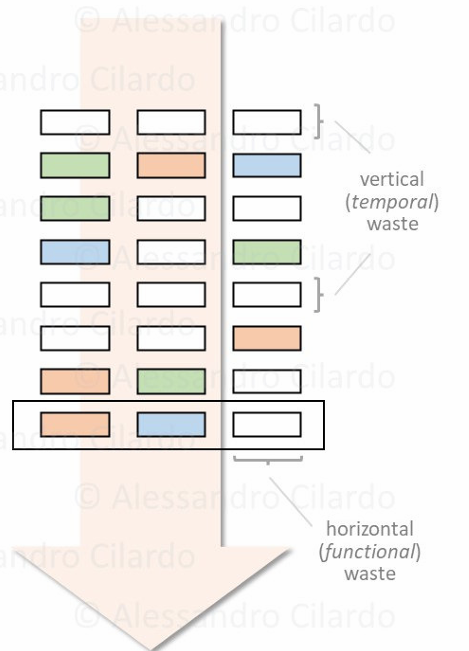
\includegraphics[width=0.29\textwidth]{fig/chapter_2/wasting.png}}
\end{figure}

Il meccanismo del multithreading simultaneo conviene perchè è possibile aumentare l'ampiezza della finestra di istruzioni recuperata (poichè i thread utilizzano istruzioni indipendenti) invece che la profondità. Si possono recuperare e accettare n istruzioni per colpo di clock, l'esecuzione è out of order e poi si possono committare fino a n istruzioni per clock. Questo risolve il problema della multiple issue. Vediamo con ordine le varie tipologie di hardware multithreading:

\begin{itemize}
    \item \textbf{Coarse-grain}: viene effettuato il cambio di contesto solo su eventi di attesa prolungata (come cache miss), e in generale su eventi che provocano sprechi verticali. Questa soluzione risulta inefficace per nascondere brevi latenze;
    \item \textbf{Fine-grain}: ad ogni colpo di clock, secondo una politica Round Robin, viene effettuato il cambio di contesto. Questa scelta è ottima perchè nasconde anche le latenze brevi e rilassa gli hazards RAW (basti pensare al fatto che vengono interlacciate istruzioni indipendenti per definizione). Questo approccio è utilizzato nelle GPU e in processori con elevato numero di thread per core;
    \item \textbf{Simultaneous multithreading}: tecnica che combina fine grain multithreading con issue multipla e scheduling dinamico. Le tecniche di \textit{register renaming} permettono a istruzioni di thread indipendenti di essere eseguito in maniera simultanea. 
\end{itemize}

\subsection{Simultaneous multithreading}
Il supporto al SMT può essere implementato \textit{on top} all'architettura pipeline vista in questo capitolo, con alcune accortezze. 
Il supporto al multithreading in un processore out-of-order si ottiene mediante la replicazione di alcune strutture architetturali fondamentali, così da garantire che ciascun thread disponga di un contesto di esecuzione autonomo. Ogni thread possiede una propria tabella di rinominazione, che costituisce il meccanismo essenziale per risolvere le dipendenze sui registri architetturali. Tale tabella associa dinamicamente i registri logici, visibili al programmatore, a registri fisici interni al processore, permettendo a thread distinti di utilizzare gli stessi identificatori senza generare conflitti. In parallelo, ogni thread mantiene un proprio Program Counter, ossia il registro che memorizza l'indirizzo dell'istruzione successiva da eseguire, il che consente al processore di prelevare istruzioni da flussi di controllo differenti in modo indipendente.
Grazie a questa duplicazione delle strutture di contesto, il processore è in grado di mantenere contemporaneamente più sequenze di istruzioni pronte per l'esecuzione. L'unità di fetch può selezionare istruzioni provenienti da thread distinti e inserirle nello stesso flusso di pipeline, mentre lo scheduling out-of-order consente di collocarle dinamicamente sulle unità funzionali disponibili, sfruttando eventuali slot altrimenti inutilizzati. In tal modo, l'esecuzione multithreaded non si riduce a una semplice alternanza temporale tra thread, ma assume la forma di una coesistenza effettiva all'interno della microarchitettura, con istruzioni appartenenti a thread diversi che avanzano in parallelo nel pipeline. L'obiettivo è incrementare il throughput globale del processore e ridurre le bolle nella pipeline, migliorando l'utilizzo delle risorse computazionali senza richiedere un incremento proporzionale del numero di core fisici.

\begin{figure}[ht]
    \centering
    \setlength{\fboxrule}{0.5pt} % spessore sottile
    \setlength{\fboxsep}{0pt}    % senza spazio interno
    \fbox{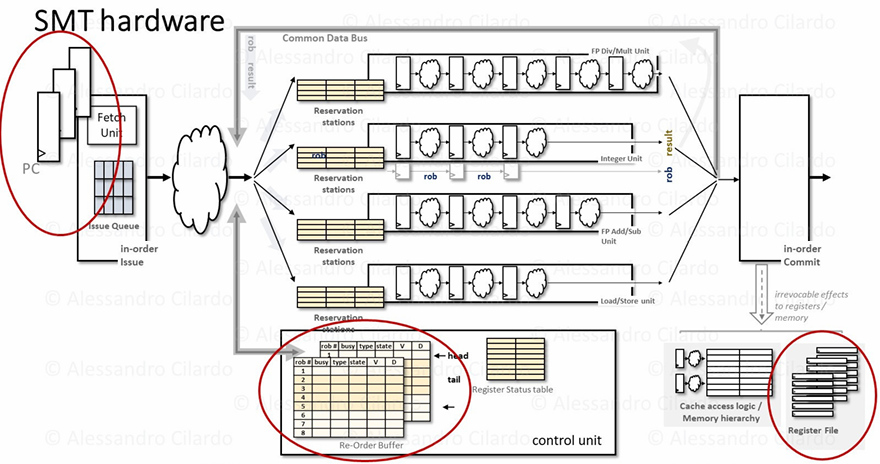
\includegraphics[width=0.9\textwidth]{fig/chapter_2/SMT.png}}
\end{figure}

\noindent Questa tecnologia hardware necessita di \textit{estendere} l'insieme di registri del processore. Infatti in un contesto multithread dobbiamo considerare che ogni thread necessita di un certo numero di registri per funzionare. In fase di esecuzione sono presenti \textit{operazioni} proveniente da istruzioni di più threads, i cui operandi sono letti e scritti da registri del processore. Questo implica una n-uplicazione dei registri del register file, e aggiungendo dei bit in più alla chiave della tabella che mantiene l'associazione nome registro $\rightarrow$ indirizzo, in modo da scriverci, in fase di issue quindi in modo totalmente trasparente all'esecuzione, l'ID del thread che sta lavorando su quel registro, e in modo che l'indirizzo del registro fisico sia univoco, nonostante più thread possano usare lo stesso registro logico. 

\noindent Quindi, anche se avviene un context switch “software” (OS), non è necessario che il processore hardware ricrei da zero ogni volta tutto il contesto dei registri se il design architetturale ha già riservato contesti separati per ogni thread logico attivo. Il vantaggio è che il passaggio fra thread hardware (SMT) può avvenire con latenza minima, senza il costo elevato di salvataggio su memoria e ricaricamento per ogni piccola alternanza tra thread. Solo quando un thread viene sospeso a livello di OS (non più residente nell’hardware) si fa il salvataggio completo dello stato.
Una delle principali complessità nella realizzazione del multithreading simultaneo riguarda la fase di commit delle istruzioni. Affinché ciascun thread possa completare correttamente e in modo indipendente la propria sequenza di istruzioni, è necessario che il processore mantenga strutture di riordino separate, spesso implementate come Reorder Buffer distinti per ogni contesto hardware. In questo modo, il ritiro delle istruzioni avviene in ordine per ciascun thread, evitando che un errore o un'eccezione in un thread influenzi la correttezza di un altro. Un'ulteriore difficoltà deriva dalla gestione della memoria condivisa: la coesistenza di thread multipli aumenta la probabilità di conflitti di cache e di fenomeni di thrashing, riducendo l'efficacia della gerarchia di memoria e degradando le prestazioni soprattutto nelle applicazioni caratterizzate da accessi intensivi e poco localizzati.

\subsection{SMT performance}
La tecnologia analizzata finora permette all'utente (di solito il sistema operativo) di vedere più \textbf{core virtuali} (o logici) per ogni core fisico. 
Nelle attuali implementazioni, l'hardware di supporto al SMT è in grado di mantenere residenti, contemporaneamente, i contesti architetturali di quattro thread diversi, ciascuno con il proprio Program Counter, i propri registri architetturali e le proprie strutture di rinominazione. In altre parole, il processore può tenere “attivi” più flussi di istruzioni, pronti a essere eseguiti. Tuttavia, il processore può prelevare e inviare istruzioni all'esecuzione solo da un thread alla volta. Ciò implica che, pur avendo più thread residenti, la fase di fetch e dispatch è monopolizzata da un singolo thread in ciascun ciclo di clock. L'unità di fetch, il decodificatore e il meccanismo di issue non combinano istruzioni provenienti da thread differenti nello stesso ciclo, ma scelgono uno dei thread disponibili e prelevano le istruzioni esclusivamente da quello. Questa è una limitazione rispetto all'SMT più “aggressivo”, dove il processore è in grado di mescolare nello stesso ciclo istruzioni provenienti da thread diversi, riempiendo le unità funzionali libere con qualunque istruzione pronta, indipendentemente dal thread di origine.

\begin{figure}[ht]
    \centering
    \setlength{\fboxrule}{0.5pt} % spessore sottile
    \setlength{\fboxsep}{0pt}    % senza spazio interno
    \fbox{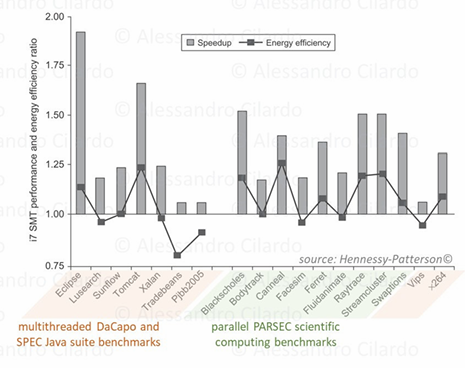
\includegraphics[width=0.5\textwidth]{fig/chapter_2/SMT_performance.png}}
\end{figure}

Dal grafico emerge che l'SMT può migliorare le prestazioni in alcuni casi, ma l'efficienza in termini energetici varia a seconda dell'applicazione. L'idea chiave è che SMT funziona meglio per alcune applicazioni rispetto ad altre, e l'efficienza energetica può essere un fattore determinante.
